\documentclass[9pt,twocolumn]{IEEEtran}
\usepackage{amsmath,amssymb,bm}
\usepackage[table]{xcolor}
\usepackage{booktabs}
\usepackage{tikz}
\usetikzlibrary{shapes.geometric,arrows.meta,positioning,calc}
\usepackage[margin=0.55in]{geometry}
\usepackage{enumitem}
\setlist{nosep,leftmargin=1.1em}

\newcommand{\pump}{\ensuremath{\mathrm{pump}}}
\newcommand{\PDN}{\ensuremath{\mathrm{PDN}}}
\newcommand{\WDN}{\ensuremath{\mathrm{WDN}}}
\newcommand{\code}[1]{\texttt{\scriptsize #1}}

\setlength{\abovedisplayskip}{2pt}
\setlength{\belowdisplayskip}{2pt}
\setlength{\textfloatsep}{4pt}
\pagestyle{empty}

\begin{document}

\title{\vspace{-2em}\normalsize How the C-OWPF Solve Modes Are Derived in Code:\\
A Transparency Note for the Companion Python Implementation}
\author{\IEEEauthorblockN{\footnotesize Companion to ``Successive Linear Approximations for Optimal
Decision Making in Interdependent Electric and Water Distribution Networks,'' IEEE Access}}
\maketitle\thispagestyle{empty}

\begin{abstract}
\footnotesize This note documents how the open-source Python implementation of the
Convex-Optimal Water-Power Flow (C-OWPF) derives each solve mode directly from the manuscript's
formulations, and maps every mode to the source that implements it. No new physics is introduced:
the code solves the same successive linear approximation of the nonlinear water hydraulics and the
LinDistFlow power model described in the paper.
\end{abstract}

\section{The Problem Solved at Each Step}
Every mode reduces to a sequence of mixed-integer convex programs of the paper's problem (P2). A
single step minimizes the priced pump energy together with the priced network loss, subject to the
linearized WDN hydraulics, the LinDistFlow PDN model, PV inverter capability, and voltage limits:
\begin{align}
\min~ & \textstyle\sum_{t}\lambda^{\WDN}_{t}\Big(\underbrace{\textstyle\sum_{ij\in\mathcal{P}}\hat{C}^{\pump}_{ij,t}}_{\text{pump energy}}
      + \underbrace{\hat{C}^{\text{loss}}_{t}}_{\text{loss}}\Big) \notag\\
\text{s.t.}~ & \text{mass balance, junction/tank/reservoir heads;} \notag\\
      & \text{lin.\ pipe head loss and (F/V)SP power;} \notag\\
      & \bm{v}^2 = \bm{R}(-\bm{p})+\bm{X}(-\bm{q})+\bm{v}_k;~ v_{\min}\!\le v_{n,t}\!\le v_{\max}. \notag
\end{align}
The pump power enters the PDN as a bus load; its reactive part is coupled through the power factor,
$q^{\pump}=p^{\pump}\tan(\arccos \mathrm{PF})$. Voltage-dependent shunt capacitors are folded into
$\bm{R},\bm{X},\bm{v}_k$ exactly as in the paper's Kekatos correction.

\section{Water (Decoupled) Solve Modes}
Four modes share the linearized hydraulics and differ only in how the operating point and pump
schedule are obtained.
\begin{itemize}
\item \textbf{EPANET} --- rule-based baseline; pumps follow tank-level rules and EPANET reports the
true nonlinear cost. No optimization; the cost reference (Scenario~A).
\item \textbf{direct} --- one linearized MILP solved once about a nominal point, no relinearization.
Fast on radial networks.
\item \textbf{warmstart} --- an EPANET-imposed schedule gives consistent flows/heads; hydraulics are
linearized \emph{once} about that point and solved. Robust on looped networks where \code{direct} fails.
\item \textbf{optimize} --- the full successive-linearization loop (Algorithm~1) wrapped in the
voltage-aware schedule search below; realizes the reported savings.
\end{itemize}

\section{Coupled Mode}
The coupled mode runs the successive-linearization loop of Fig.~\ref{fig:flow} and then a schedule
search that, unlike the water-only search, scores every candidate on the \emph{coupled} solve, so a
schedule that is cheap for water yet causes an undervoltage on the feeder is rejected.

\smallskip\noindent\textbf{Schedule search is cost- and voltage-aware:} each candidate is scored on
the true total cost (pump $+$ loss) and voltage feasibility.

\smallskip\noindent\textbf{Warm-started trust-region MILP:} free binaries, warm-started at the
incumbent's linearisation, with a Hamming-distance cap of $K$ flips --- the MATLAB-style free-binary
MILP made reliable (the trust region blocks the far-away schedule flips a cold MILP would take on a
stale linearisation).

\smallskip Concretely the search runs in four stages, ranking \emph{coupled-feasible first} (water
slack and voltage violation within tolerance), then lowest true cost: (1)~EPANET baseline;
(2)~price-quantile candidates --- pump only in the cheapest hours (plus a duty-preserving load shift
on large networks); (3)~warm-started trust-region MILP, $K=\max(2,\lfloor n_{\pump}T/4\rfloor)$;
(4)~$1$-opt polish (single pump-hour flips, greediest-price first).

\section{Validation}
The winning schedule is never trusted on its linear score alone: the water schedule is replayed in
\textbf{EPANET} ($\Delta H$, $\Delta$flow) and the power injections in the nonlinear \textbf{Z-bus}
fixed-point solver (true voltages and true $\sum |I|^2 r$ loss).

\begin{figure}[t]
\centering
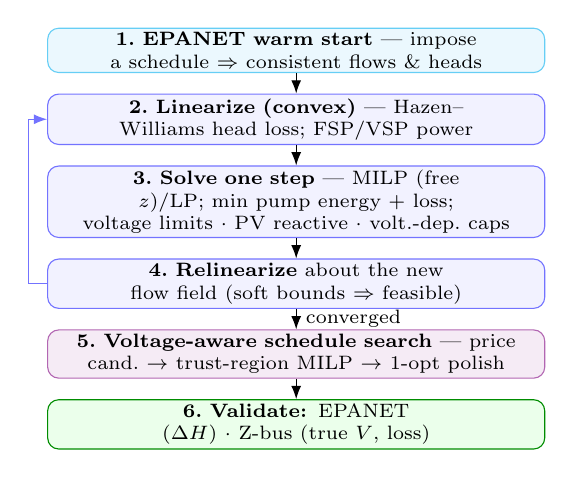
\begin{tikzpicture}[
  font=\scriptsize,>=Latex,node distance=2.6mm,
  box/.style={rounded corners,draw,align=center,inner sep=1.6pt,minimum height=5.6mm,text width=62mm},
  loop/.style={box,draw=blue!55,fill=blue!5},
  warm/.style={box,draw=cyan!60,fill=cyan!8},
  sch/.style={box,draw=violet!60,fill=violet!8},
  val/.style={box,draw=green!55!black,fill=green!8}]
\node[warm] (a) {\textbf{1.\ EPANET warm start} --- impose a schedule $\Rightarrow$ consistent flows \& heads};
\node[loop,below=of a] (b) {\textbf{2.\ Linearize (convex)} --- Hazen--Williams head loss; FSP/VSP power};
\node[loop,below=of b] (c) {\textbf{3.\ Solve one step} --- MILP (free $z$)/LP; min pump energy $+$ loss;\\ voltage limits $\cdot$ PV reactive $\cdot$ volt.-dep.\ caps};
\node[loop,below=of c] (d) {\textbf{4.\ Relinearize} about the new flow field (soft bounds $\Rightarrow$ feasible)};
\node[sch,below=of d] (e) {\textbf{5.\ Voltage-aware schedule search} --- price cand.\ $\to$ trust-region MILP $\to$ 1-opt polish};
\node[val,below=of e] (f) {\textbf{6.\ Validate:} EPANET ($\Delta H$) $\cdot$ Z-bus (true $V$, loss)};
\draw[->](a)--(b); \draw[->](b)--(c); \draw[->](c)--(d);
\draw[->,blue!55] (d.west) -- ++(-2.4mm,0) |- ($(b.west)+(-2.4mm,0)$) -- (b.west);
\draw[->](d)--(e) node[midway,right]{converged}; \draw[->](e)--(f);
\end{tikzpicture}
\caption{The coupled C-OWPF solve. Steps 2--4 are the successive-linearization loop; step~5 wraps it
in the cost- and voltage-aware schedule search.}
\label{fig:flow}
\end{figure}

\section{Code Map}
All paths are under \code{Python/}.
\begin{table}[h]
\centering\renewcommand{\arraystretch}{1.05}
\begin{tabular}{@{}ll@{}}
\toprule
{\scriptsize Element} & {\scriptsize Source} \\
\midrule
{\scriptsize Water modes / driver}       & \code{main\_owf.py: MODES, run\_case} \\
{\scriptsize Succ.\ lin.\ + search}       & \code{owf/warmstart.py: optimize\_schedule} \\
{\scriptsize Price / load-shift cand.}    & \code{owf/warmstart.py: price\_threshold\_schedules} \\
{\scriptsize Coupled step (P2)}           & \code{coupled/coupled\_lp.py: solve\_coupled} \\
{\scriptsize Trust region $(z_0,K)$}       & \code{coupled/coupled\_lp.py: build\_coupled\_problem} \\
{\scriptsize Coupled sched.\ search}       & \code{coupled/schedule.py: optimize\_coupled\_schedule} \\
{\scriptsize LinDistFlow / branch flows}  & \code{pdn/lindistflow.py: build\_lindist} \\
{\scriptsize Nonlinear validation}        & \code{coupled/validation.py (Z-bus) + EPANET} \\
\bottomrule
\end{tabular}
\end{table}

\end{document}
